\documentclass[runningheads,a4paper]{llncs}
\usepackage{amssymb}
\setcounter{tocdepth}{3}
\usepackage{graphicx}
\usepackage{subfigure}
\usepackage{url}
\usepackage{color}
%\usepackage{verbatim}
%\usepackage{pgfplots}
\usepackage{bbding}
\usepackage{multirow}
\urldef{\mailsa}\path|{alfred.hofmann, ursula.barth, ingrid.haas, frank.holzwarth,|
\urldef{\mailsb}\path|anna.kramer, leonie.kunz, christine.reiss, nicole.sator,|
\urldef{\mailsc}\path|erika.siebert-cole, peter.strasser, lncs}@springer.com|
\newcommand{\keywords}[1]{\par\addvspace\baselineskip
\noindent\keywordname\enspace\ignorespaces#1}
\setlength{\parskip}{0.2\baselineskip}
\begin{document}

\mainmatter  % start of an individual contribution

% first the title is needed
\title{Dual-Convolutional Enhanced Residual Network for Single Super-Resolution of Remote Sensing Images}

% a short form should be given in case it is too long for the running head
\titlerunning{DCER for SR of Remote Sensing Images}
\author{Xuewei Li\inst{1} \and
Hongqian Shen\inst{1} \and
Chenhan Wang\inst{2}\and Han Jiang\inst{2} \and Ruiguo Yu\inst{1}\Envelope \and Jianrong Wang\inst{1} \and Mankun Zhao\inst{1}}
%
\authorrunning{Ruiguo Yu et al.}

\institute{
School of Computer Science and Technology, Tianjin University, China\\
\email{\{lixuewei,hongqianshen,rgyu,wjr,zmk\}@tju.edu.cn}
\and
Beijing AXIS Technology Company Limited, China\\
\email{\{gabriel,hahn\}@signcl.com}
}

\maketitle


\begin{abstract}
The image super-resolution aims to recover a high-resolution image using a single or sequential low-resolution images. The super resolution methods based on deep learning, especially the deep convolutional neural network, have achieved good results. In this paper,we propose Dual-Convolutional Enhanced Residual Network (DCER) for remote sensing images based on residual learning, which concatenates the feature maps of different convolutional kernel sizes (3x3, 5x5). On the one hand, it can learn more high-frequency detail information by combining the local details of different scales; on the other hand, it reduces network parameters and greatly shorten the training time. The experimental results show that DCER achieves favorable performance of accuracy and visual performance against the state-of-the-art methods with the scale factor 2x,4x and 8x.
\keywords{Dual-Convolutional Enhanced Residual Network(DCER); Single Super-Resolution; Remote Sensing Images}
\end{abstract}


\section{Introduction}
High-resolution(HR) images contain more information and better accuracy, which is helpful to the further mining, understanding and processing of image contents. The spatial resolution of the satellite remote sensing image depends on the accuracy of the sensor, and the improvement of the performance of the imaging system is accompanied with an expensive manufacturing cost. Super-resolution(SR) \cite{Kolte2013Image} is to use a single or sequential low-resolution(LR) images with complementary information to obtain high-resolution images, which is of great significance to improve image quality.

At present, there are many researches on super-resolution of images. The super-resolution technology is divided into three categories: interpolation, multi-frame reconstruction and learning-based methods.The early interpolation method \cite{1163154} generally uses an interpolation kernel to estimate the value of an unknown pixel in a high-resolution grid. Because the interpolation kernel cannot adapt to the image and does not introduce effective high-frequency information. Therefore, the upsampled image is easy to blur, and many sharp edge details cannot be retained. The super-resolution technology based on multi frame reconstruction\cite{872908,IRANI1991231,56062,Patti1997Superresolution,503915} uses the prior information of the image to establish a mathematical model or gradually improve the HR by using an iterative method. Due to the need to fuse information from multiple frames of LR, the applicability and accuracy of the motion model will greatly affect the reconstruction effect.The learning-based super-resolution  algorithm\cite{Shu2013Example,Yang2008Image} searches for the mapping relationship between LR and the corresponding HR image by the training dataset, and finds the optimal solution for LR.

Recently, with the development of deep neural networks, Dong et al. \cite{Dong2014Learning} proposed a Super-Resolution Convolutional Neural Network(SRCNN) with three convolutional layers for SR. Kim et al. \cite{Kim2015Accurate} proposed a Very Deep Convolutional Networks(VDSR),which increased the network depth by cascading small filters and learning residuals. But since both SRCNN \cite{Dong2014Learning} and VDSR \cite{Kim2015Accurate} need to use the bicubic interpolation as the upsampling operator to enlarge images to the size of the target, thus it increased the unnecessary computing cost. Dong et al. \cite{Dong2016Accelerating} proposed Accelerating the super-resolution convolutional
neural network (FSRCNN) to construct the SR images at the last step by  deconvolution. Kim et al. \cite{Kim2015Deeply} used a deep recursive neural network which got better performance at a small number of parameters. Kolte et al. \cite{Lai2017Deep} used the Laplacian Pyramid
Super-Resolution Network (LapSRN) to progressively  extract features and carry out upsampling, which then computed the output of the previous layer into the loss function, and supervised the results of each stage. Ledig et al.\cite{Ledig2016Photo} used 16 blocks deep ResNet(SRResNet) to construct loss function, Lim et al.\cite{Lim2017Enhanced} proposed Enhanced deep residual networks (EDSR) which also applied residual network for SR. EDSR\cite{Lim2017Enhanced} removed  batch normalization  from SPResNet\cite{Ledig2016Photo}, simplifying the network while improving its performance, which won the championship in the NTIRE2017 Super Resolution Challenge.

Multi-frame reconstruction has been widely used in remote sensing image SR \cite{Li2015Super,Zhang2014Super}, and multi-frame reconstruction needs to obtain multiple images of the same scene. However, in many specific satellite applications, multiple images of the same scene are difficult to obtain because of the different angle and resolution of the sensor, or the long revisit time of the same sensor. Therefore, single frame SR is more suitable for remote sensing. The traditional based on learning method\cite{Yang2010Image} is mostly based on low-level feature design, and reconstruction results are poor in complex space remote sensing images. Therefore,Dual-Convolutional Enhanced Residual Network (DCER) is proposed to better reconstruct super-resolution images by combining local image details at different scales.


The main contributions of this paper can be summarized in the following two points:

(1) DCER is applied to the single super-resolution of  remote sensing images to enhance the details of remote sensing images.

(2) DCER with different convolutional kernels(3x3, 5x5) can combine the local details of different scales, and uses 1x1 convolutional layer to reduce the dimensions, and speed up network training.


\section{Related Works}
In recent years, the deep neural network, after a rapid development, has shown its superior capability in the field of computer vision. Dong et al.\cite{Dong2014Learning}  first proposed SRCNN for SR, and established the end-to-end mapping between LR and HR. SRCNN consists of three operations:patch extraction and representation,non-linear mapping and reconstruction. As the network deepens, the advanced features learned on the one hand will become much more. On the other hand, the correlation between gradients in backward propagation will become increasingly worse, and the degradation of the network will lead to greater errors. He et al.\cite{He2015Deep} presented a residual learning framework to train deeper networks. The Residual block was implemented by shortcut connection to stack the input and output. Adding element-wise overlays does not add extra parameters and computational complexity to the network. When the number of  network layers increases, the residual learning framework can solve the gradient disappearance and over fitting problem of deep convolutional network.


SRResnet \cite{Ledig2016Photo}and EDSR \cite{Lim2017Enhanced} applied a residual learning to the super resolution. Each residual block structure in SRResnet \cite{Ledig2016Photo} has two convolutional layers. The batch normalization and Relu activation functions are used between the convolutional layers. Batch normalization is to process the mean and variance of each training batch data with the addition of translation and scaling parameters, but it destroys the spatial information of the image to a certain extent and offsets the gain brought about by the network depth. Given that, EDSR  \cite{Lim2017Enhanced} removed batch normalized modules in the residual structure. Since the batch normalization layer consumes memory,  after removing the batch normalization, EDSR \cite{Lim2017Enhanced} stacks more convolutional layers and extracts more features at each layer, resulting in better performance. The final version of EDSR\cite{Lim2017Enhanced} has 32 residual blocks, each convolutional layer with 256 channels.The huge amount of network parameters leads to a slow network training. For upsampling factor 3x and 4x, initializing model parameters with pre-trained 2x network parameters.Even though this can reduce the training time of the high upsampling factor model, the network training time per epoch still takes a lot of time.

Increasing the depth or width of the network model will inevitably increase the computational complexity. In order to prevent over-fitting and increased computational complexity, Szegedy et al.\cite{Szegedy2014Going} proposed an efficient deep neural network architecture called GoogLeNet. The core of the GoogLeNet architecture is the Inception module, with a depth of 22 layers. In terms of model depth, in order to avoid the problem of gradient disappearance, GoogLeNet increases two loss at different depths; and when it comes to the width of the model, the Inception architecture consists of filter sizes 1x1,3x3,5x5. With different sizes of convolutional kernels, the sizes of the receptive fields are also different, and the final splicing merges features of different scales. Concating the feature maps of different convolutional kernel sizes fuses local detail information. In order to reduce the huge computational complexity of the 5x5 convolutional kernel, the 1x1 convolutional kernel is used for dimensionality reduction, and then multi-scale convolution is performed separately.Therefore, the Inception  not only improves the ability of convolution to extract features, but also eases the bottleneck of computing resources.

This paper is based on the use of multi-scale convolutional filters  to improve EDSR \cite{Lim2017Enhanced} , shorten the network training time, and achieve excellent performance.

\section{Proposed Methods}
In this section, we will specifically describe the proposed DCER network  and the training details of the network.

\subsection{Dual-Convolutional Enhanced Residual Networks}

The EDSR \cite{Lim2017Enhanced} has been applied to super resolution which has achieved excellent results. It has restored image details better than other methods.The application of residual learning in EDSR \cite{Lim2017Enhanced} increases the number of network layers, and at the same time, more convolutional kernels are used on each layer, resulting in a huge amount of parameters. To solve this problem, we proposes Dual-Convolutional Enhanced Residual Networks. In Fig. 1, (a) is the residual block of EDSR\cite{Lim2017Enhanced}, and (b) is the residual block presented in this paper.Firstly, we change the single 3x3 convolutional kernel to the 3x3 and 5x5 convolutional kernels to jointly extract features. Secondly, after the Relu activation, 1x1 convolutional kernel is used to reduce the dimension of the previous 256 features to 64.Then, two convolutional operations are respectively performed using 3x3, 5x5 dual-channel networks, and finally feature fusion is performed. Comparing the parameter quantities of a block (only calculating the convolutional weight parameters and ignoring the deviation parameters), EDSR\cite{Lim2017Enhanced} has 1179648 parameters and DCER has 851968 parameters, so in a residual block, DCER reduces the parameter amount of about 21.78\%.

\begin{figure}[htbp]
\centering
\subfigure[ EDSR]{
    \begin{minipage}{4cm}
    %\centering
    \includegraphics[width=150px,height=200px]{pic/1.png}
    \end{minipage}
}
\hspace{1cm}
\subfigure[Proposed]{
    \begin{minipage}{6cm}
    %\centering
    \includegraphics[width=150px,height=200px]{pic/2.png}
    \end{minipage}
}
\caption{Comparison of residual blocks in EDSR and ours }
\label{res}
\end{figure}
As for the network depth, the deeper the network is, the greater the receptive field is, that is, the larger the mapping range of the output result is, the higher the globality and the abstractness are. Deep networks are mostly used for image classification and  recognition. For super-resolution, no specific features and high abstract features are needed to determine the final output. On the other hand, as network layers deepen, the network model is likely to degenerate and reduce the effective dimension of the model. So this paper sets up 16 residual blocks for network. The overall network structure is shown in Fig. 2.

\begin{figure}
\centering
\includegraphics[scale=0.4]{pic/network.png}
\caption{The architecture of the proposed DCER network structure.A low-resolution image goes through the first convolutional layer,and then enters 16 residual learning blocks.The high-resolution image is obtained by transposed convolutions  }
\label{fig:example}
\end{figure}

\subsection{Training Details}
During the training phase, we downsample high-resolution images to corresponding low-resolution images, which form training-label sample pairs. The sample size and total number of different sampling times can be referred to in Sec. 4.1. The activation function is Relu. Batchsize is 2. The initial learning rate is set to 0.001, with inverse time decay, setting the globalstep to 2500. The loss function uses L1 Loss. Although the mean squared error is the most important measure used in image quality assessment, the image output by minimizing the mean squared error is too smooth, and the PSNR could not effectively capture the complex features of the human visual system\cite{Zhang2012A}. All experiments are carried on an Inter E5-2690 CPU 2.6GHz with 188 GB RAM and Tesla K80  using the tensorflow package.

\section{Experiments}
\subsection{Datasets}

The experimental data in this paper is remote sensing image with spatial resolution of 1.07m/pixel provided by Beijing AXIS Technology Company Limited. According to the spectral response of the objects, three channels are selected to synthesize three channels of RGB images. The image segmentation step is based on the image size, ensuring that there is no cross between images. The segmented image randomly selects 20\% as the testing set and the rest is the training set. In the experiment, considering the size of the image after x8 upsampling,we reduce the size of original image,so the image input sizes of different upsampling factors are different,as shown in Table 1. All images are down-sampled to get the corresponding low-resolution image.

\begin{table}
\caption{Dataset of different up sampling factor}
\centering
\begin{tabular}{cccc}
\hline\noalign{\smallskip}
scale &  \quad LR size &  \quad training samples &  \quad testing samples\\
\noalign{\smallskip}
\hline
\noalign{\smallskip}
x2 &  \quad64x64 &  \quad13600 &  \quad3400\\
x4 &  \quad64x64 &  \quad10000 &  \quad2500\\
x8 &  \quad32x32 &  \quad10000 &  \quad2500\\
\hline
\end{tabular}
\label{compare}
\end{table}

\subsection{Comparisons with the state-of-the-arts}
To comfirm the ability of the proposed network, we compare our network with four state-of-the-art SR algorithms:Bicubic, SRCNN\cite{Dong2014Learning}, VDSR\cite{Kim2015Accurate}, EDSR\cite{Lim2017Enhanced}. The quantitative results with the scale factor 2x,4x and 8x are shown in the Table 2. Image reconstruction quality uses PSNR and SSIM as two evaluation indicators, and PSNR calculation method is as shown in formula (1) and formula (2).MAX is 255, and C, H, and W are the number of channels, height, and width of the image, respectively. X(i,j,k) and Y(i,j,k) represent network output results and high-resolution image pixel values. Among these methods,DCER has the best performance with the highest PSNR and SSIM over 2,4,8 scale. We
also present the qualitative results in Fig. 3. By visual comparison, DCER performs well in SR applications of remote sensing images. Compared with other methods, the edges of the HR images obtained by DCER are clear, and the details of the image texture are obviously enhanced, and the edge structure features of the images are well preserved.
\begin{small}
\begin{equation}
  PSNR = 10\times lg(\frac{MAX^2}{MSE})
\end{equation}
\begin{equation}
  MSE = \frac{1}{C\times H\times W}\times\sum_{i=1}^C\sum_{j=1}^H\sum_{k=1}^W \left ||X(i,j,k)-Y(i,j,k) \right ||^2
\end{equation}
\end{small}

\begin{table}

\caption{Mean PSNR(dB) and SSIM over different scale}
\centering
\begin{tabular}{cccccc}
\hline\noalign{\smallskip}

\multirow{2}{*}{scale} & \quad Bicubic&  \quad SRCNN & \quad VDSR &  \quad EDSR& \quad DCER  \\
&\quad PSNR/SSIM&  \quad PSNR/SSIM & \quad PSNR/SSIM &  \quad PSNR/SSIM& \quad PSNR/SSIM  \\

\noalign{\smallskip}
\hline
\noalign{\smallskip}
x2 & \quad 31.366 /0.87&\quad 32.037/0.88&\quad 32.977/0.90&\quad 33.975/0.91&\textbf{\quad34.155/0.92}\\
x4 & \quad 26.503 /0.70 &\quad 27.443/0.71&\quad 28.077/0.74&\quad 28.880/0.77&\textbf{\quad 29.000/0.78}\\
x8 & \quad 21.989/0.48 &\quad 24.182/0.54&\quad 24.501/0.56&\quad 26.053/0.63&\textbf{\quad 26.098/0.64}\\
\hline
\end{tabular}
\label{compare}
\end{table}
\begin{figure}[htbp]

    \begin{minipage}{1.3cm}
    \includegraphics[scale=0.4]{pic/2x/hr/518.png}
    \includegraphics[scale=0.8]{pic/2x/hr/small-518.png}
    {HR \linebreak PSNR\linebreak SSIM}
    \end{minipage}
    \qquad
    \begin{minipage}{1.4cm}
    \includegraphics[scale=0.4]{pic/2x/bicu/pick-518.png}
    \includegraphics[scale=0.8]{pic/2x/bicu/small-518.png}
    {Bicubic \linebreak 29.174dB\linebreak 0.881}
    \end{minipage}
    \qquad
    \begin{minipage}{1.3cm}
     \includegraphics[scale=0.4]{pic/2x/srcnn/pick-518.png}
    \includegraphics[scale=0.8]{pic/2x/srcnn/small-518.png}
    {SRCNN \newline29.198dB\newline 0.883}
    \end{minipage}
    \qquad
    \begin{minipage}{1.3cm}
    %\centering
     \includegraphics[scale=0.4]{pic/2x/vdsr/pick-518.png}
    \includegraphics[scale=0.8]{pic/2x/vdsr/small-518.png}
    {VDSR \newline32.038dB\newline 0.922}
    \end{minipage}
    \qquad
    \begin{minipage}{1.3cm}
    %\centering
     \includegraphics[scale=0.4]{pic/2x/edsr/pick-518.png}
    \includegraphics[scale=0.8]{pic/2x/edsr/small-518.png}
    {EDSR \newline31.813dB\newline 0.927}
    \end{minipage}
    \qquad
    \begin{minipage}{1.3cm}
    %\centering
    \includegraphics[scale=0.4]{pic/2x/dcer/pick-518.png}
    \includegraphics[scale=0.8]{pic/2x/dcer/small-518.png}
    {DCER \newline32.327dB\newline0.932}
    \end{minipage}
    \qquad
    \begin{minipage}{1.3cm}
    \includegraphics[scale=0.2]{pic/4x/hr/35.png}
    \includegraphics[scale=0.8]{pic/4x/hr/small-35.png}
    {HR \newline PSNR\newline SSIM}
    \end{minipage}
    \qquad
    \begin{minipage}{1.3cm}
    \includegraphics[scale=0.2]{pic/4x/bicu/pick-35.png}
    \includegraphics[scale=0.8]{pic/4x/bicu/small-35.png}
    {Bicubic \newline 23.295dB\newline0.620}
    \end{minipage}
    \qquad
    \begin{minipage}{1.4cm}
     \includegraphics[scale=0.2]{pic/4x/srcnn/pick-35.png}
    \includegraphics[scale=0.8]{pic/4x/srcnn/small-35.png}
    {SRCNN \newline23.793dB\newline0.621}
    \end{minipage}
    \qquad
    \begin{minipage}{1.3cm}
     \includegraphics[scale=0.2]{pic/4x/vdsr/pick-35.png}
    \includegraphics[scale=0.8]{pic/4x/vdsr/small-35.png}
    {VDSR \newline24.260dB\newline0.644}
    \end{minipage}
    \qquad
    \begin{minipage}{1.3cm}
     \includegraphics[scale=0.2]{pic/4x/edsr/pick-35.png}
    \includegraphics[scale=0.8]{pic/4x/edsr/small-35.png}
    {EDSR \newline 26.075dB \newline0.749}
    \end{minipage}
    \qquad
    \begin{minipage}{1.3cm}
    \includegraphics[scale=0.2]{pic/4x/dcer/pick-35.png}
    \includegraphics[scale=0.8]{pic/4x/dcer/small-35.png}
    {DCER \newline26.496dB\newline0.768}
    \end{minipage}
    \qquad
    \begin{minipage}{1.4cm}
    %\centering
    \includegraphics[scale=0.2]{pic/8x/hr/437.png}
    \includegraphics[scale=0.8]{pic/8x/hr/small-437.png}
    {HR \newline PSNR\newline SSIM}
    \end{minipage}
    \qquad
    \begin{minipage}{1.4cm}
    %\centering
    \includegraphics[scale=0.2]{pic/8x/bicu/pick-437.png}
    \includegraphics[scale=0.8]{pic/8x/bicu/small-437.png}
    {Bicubic \newline 22.735dB \newline0.533}
    \end{minipage}
    \qquad
    \begin{minipage}{1.5cm}
    %\centering
     \includegraphics[scale=0.2]{pic/8x/srcnn/pick-437.png}
    \includegraphics[scale=0.8]{pic/8x/srcnn/small-437.png}
    {SRCNN \newline 24.954dB \newline 0.595}
    \end{minipage}
    \qquad
    \begin{minipage}{1.4cm}
    %\centering
     \includegraphics[scale=0.2]{pic/8x/vdsr/pick-437.png}
    \includegraphics[scale=0.8]{pic/8x/vdsr/small-437.png}
    {VDSR \newline 24.964dB\newline 0.616}
    \end{minipage}
    \qquad
    \begin{minipage}{1.4cm}
    %\centering
     \includegraphics[scale=0.2]{pic/8x/edsr/pick-437.png}
    \includegraphics[scale=0.8]{pic/8x/edsr/small-437.png}
    {EDSR \newline 26.926dB \newline0.689}
    \end{minipage}
   \qquad
    \begin{minipage}{1.3cm}
    %\centering
    \includegraphics[scale=0.2]{pic/8x/dcer/pick-437.png}
    \includegraphics[scale=0.8]{pic/8x/dcer/small-437.png}
    {DCER \newline 27.593dB\newline 0.705}
    \end{minipage}

\caption{Qualitative comparsion of our models with other works on scale different super-resolution,2x,4x,8x upsampling from top to bottom}
\label{res}
\end{figure}
\subsection{Network Parameters and Training Time}
DCER is improved based on the network structure of EDSR\cite{Lim2017Enhanced}. In this section, we analyze the network parameter settings of EDSR \cite{Lim2017Enhanced} and DCER ,and compare the parameter capacity. In addition, referring to the EDSR\cite{Lim2017Enhanced} paper and code, we implement and apply the data set of this paper to train and test the model. By reason of diverse the input sizes of different sampling multiple networks , we list the number of model parameters of different sampling factors, time of each epoch training  and their corresponding  training results, as shown in Table 3.

\begin{table}
\caption{Comparison of parameters and training time}
\centering
\begin{tabular}{ccccc}
\hline\noalign{\smallskip}
scale & \quad method &  \quad parameters & \quad training time/epoch(min) & \quad mean PSNR(dB)  \\
\noalign{\smallskip}
\hline
\noalign{\smallskip}
x2 & \quad EDSR &\quad 1179648 &\quad 85.11&\quad 33.975\\
x2 & \quad DCER &\quad 854968&\quad 60.05&\quad 34.155\\
x4 & \quad EDSR &\quad 1179648 &\quad 65.05&\quad 28.880\\
x4 & \quad DCER &\quad 854968 &\quad 40.04&\quad 29.000\\
x8 & \quad EDSR &\quad 1179648&\quad 21.32&\quad 26.053\\
x8 & \quad DCER &\quad 854968&\quad 11.20&\quad 26.098\\
\hline
\end{tabular}
\label{compare}
\end{table}
In the training process, we test all the test data after each  training epoch to observe the training result. As shown in Fig. 4, comparing the training/test results of EDSR\cite{Lim2017Enhanced} and DCER at different sampling factor per epoch, it can be clearly seen that DCER can reach a steady trend quickly, and is higher than EDSR\cite{Lim2017Enhanced} in each round of PSNR evaluation indicators. This illustrates the effectiveness of DCER network extraction features.

\begin{figure}[htbp]
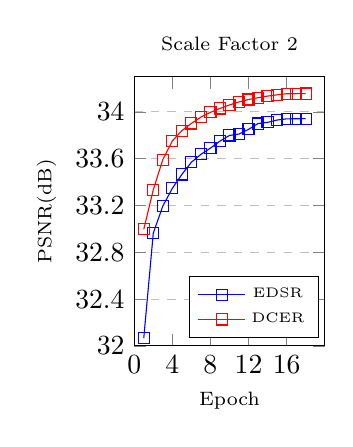
\begin{tikzpicture}
\begin{axis}[
    title={ \scriptsize Scale Factor 2},
    xlabel={ \scriptsize Epoch},
    ylabel={ \scriptsize PSNR(dB)},
    xmin=0, xmax=20,
    ymin=32, ymax=34.3,
    xtick={ 0,4,8,12,16},
    ytick={ 32.0,32.4,32.8,33.2,33.6,34.0},
    legend pos=south east,
    ymajorgrids=true,
    grid style=dashed,
    width=4cm,height=5cm,]
    \addplot[
    color=blue,
    mark=square,
    ]
    coordinates{
    (1,32.0655)(2,32.96373558)(3,33.194658)(4,33.345991)(5,33.464778)(6,33.56919)(7,33.63676)(8,33.69)
    (9,33.75)(10,33.798)(11,33.81)(12,33.85)(13,33.9)(14,33.91)(15,33.93)(16,33.94)(17,33.941)(18,33.942)
    };
    \addlegendentry{\tiny EDSR}
    \addplot[
    color=red,
    mark=square,
    ]
    coordinates{
    (1,32.9965)(2,33.33379)(3,33.59179)(4,33.751)(5,33.83936)(6,33.90089)(7,33.955)(8,33.9956)
    (9,34.02886)(10,34.059)(11,34.0847)(12,34.10546)(13,34.12044)(14,34.13439)(15,34.14525)(16,34.15472)(17,34.155)(18,34.156)
    };
    \addlegendentry{\tiny DCER}
\end{axis}
\end{tikzpicture}
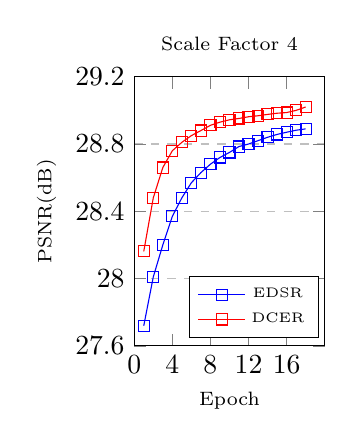
\begin{tikzpicture}
\begin{axis}[
    title={ \scriptsize Scale Factor 4},
    xlabel={ \scriptsize Epoch},
    ylabel={ \scriptsize PSNR(dB)},
    xmin=0, xmax=20,
    ymin=27.6, ymax=29.2,
    xtick={0,4,8,12,16},
    ytick={27.6,28.0,28.4,28.8,29.2},
    legend pos=south east,
    ymajorgrids=true,
    grid style=dashed,
    width=4cm,height=5cm,]
    \addplot[
    color=blue,
    mark=square,
    ]
    coordinates{
    (1,27.72)(2,28.01)(3,28.20)(4,28.37)(5,28.48)(6,28.57)(7,28.63)(8,28.68)
    (9,28.72)(10,28.75)(11,28.785)(12,28.80)(13,28.82)(14,28.84)(15,28.857)(16,28.870)(17,28.882)(18,28.89)
    };
    \addlegendentry{\tiny EDSR}
    \addplot[
    color=red,
    mark=square,
    ]
    coordinates{
    (1,28.162)(2,28.48)(3,28.66)(4,28.76)(5,28.81)(6,28.85)(7,28.88)(8,28.911)
    (9,28.93)(10,28.944)(11,28.952)(12,28.962)(13,28.968)(14,28.976)(15,28.983)(16,28.987)(17,29)(18,29.02)
    };
    \addlegendentry{\tiny DCER}
\end{axis}
\end{tikzpicture}
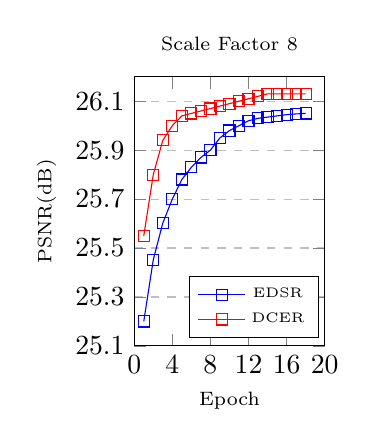
\begin{tikzpicture}
\begin{axis}[
    title={ \scriptsize Scale Factor 8},
    xlabel={ \scriptsize Epoch},
    ylabel={ \scriptsize PSNR(dB)},
    xmin=0, xmax=20,
    ymin=25.1, ymax=26.2,
    xtick={0,4,8,12,16,20},
    ytick={25.1,25.3,25.5,25.7,25.9,26.1},
    legend pos=south east,
    ymajorgrids=true,
    grid style=dashed,
    width=4cm,height=5cm,]
    \addplot[
    color=blue,
    mark=square,
    ]
    coordinates{
    (1,25.2)(2,25.452)(3,25.602)(4,25.7)(5,25.78)(6,25.83)(7,25.87)(8,25.90)
    (9,25.95)(10,25.98)(11,26)(12,26.02)(13,26.03)(14,26.035)(15,26.04)(16,26.045)(17,26.048)(18,26.05)
    };
    \addlegendentry{ \tiny EDSR}
    \addplot[
    color=red,
    mark=square,
    ]
    coordinates{
    (1,25.55)(2,25.8)(3,25.94)(4,26)(5,26.04)(6,26.05)(7,26.06)(8,26.07)
    (9,26.08)(10,26.09)(11,26.1)(12,26.11)(13,26.12)(14,26.13)(15,26.13)(16,26.13)(17,26.13)(18,26.13)
    };
    \addlegendentry { \tiny DCER}
\end{axis}
\end{tikzpicture}


\caption{Qualitative comparison of the results of EDSR and DCER(our models) on each training  epoch }
\label{res}
\end{figure}
\section{Conclusion}
In this paper, we propose a Dual-Convolutional Enhanced Residual network for single super-resolution of Remote Sensing Images. DCER combines different scale features in the basic blocks, and uses local residual learning between each module to improve the model degradation caused by the depth of the network. During  training and testing models on remote sensing image datasets, compared with other methods, DCER has achieved very good results. In particular, when compared to the EDSR\cite{Lim2017Enhanced} and DCER training process in each epoch, DCER has a stronger ability to extract features and can achieve overall fast convergence.
\bibliographystyle{splncs03}
\bibliography{ref}
\end{document}
